%! Tex program = pdflatex
 
\documentclass[UTF8]{ctexart}
\CTEXsetup[format={\Large\bfseries}]{section}
\usepackage{amsmath}
\usepackage{ctex}
\usepackage{array}
\usepackage{ulem}
\usepackage{graphicx}
\usepackage{geometry}
\usepackage{multirow}
\usepackage{subfig}
\usepackage{float}
\usepackage{multicol}
\usepackage{multirow}
\usepackage{indentfirst}
\usepackage{makecell}
\geometry{papersize={21cm,29.7cm}}
\geometry{left=2.54cm,right=2.54cm,top=3.18cm,bottom=3.18cm}
\usepackage{fancyhdr}
\pagestyle{fancy}
\lhead{\today}
\chead{}
\rhead{2020011075}
\lfoot{清华大学}
\cfoot{\thepage}
\rfoot{智能传感与检测技术}
\renewcommand{\headrulewidth}{0.4pt}
\renewcommand{\headwidth}{\textwidth}
\renewcommand{\footrulewidth}{0pt}
\usepackage{bm}
\begin{document}
\begin{titlepage}
    \begin{center}
		\quad \\
		\quad \\
        \quad \\
        \quad \\
        \quad \\
        \quad \\
		\kaishu \fontsize{30}{15} 基于梯度张量测量仪的磁法探测\\实验报告

	\end{center}
	\vskip 10cm

    \begin{center}
        \begin{large}
        \begin{tabular}{cc}
        院\qquad 系:& ~~~~~~~~自动化系~~~~~~~~      \\
        \cline{2-2}\\
        班\qquad 级:& 自02班   \\
        \cline{2-2}\\
        学生姓名:& 彭程    \\
        \cline{2-2}\\
        学\qquad 号:&2020011075   \\
        \cline{2-2}
        \end{tabular}
        \end{large}
        \end{center}

\end{titlepage}
\newpage
\tableofcontents
\newpage
\section{实验名称}
基于梯度张量测量仪的磁法探测
\section{实验目的}
\begin{enumerate}
\item 了解磁法探测的原理和方法。
\item 了解磁场梯度探测仪的结构和功能。
\end{enumerate}

\section{实验原理}
在地球表面一个相对很小的局部区域,在没有磁异常的情况下,用磁力仪测
量得出的磁力线是平行分布的。

在地下有铁磁性目标埋藏时,由于铁磁性目标被磁化,局部区域内产生磁异
常,用磁力仪进行观测,就能发现磁异常的范围和强度情况。通过
对观测数据的反演解释,即可推测得到地下目标的埋藏位置、大小等参数。
    
本次实验中,采用磁法探测的磁偶极子定位方法,常用的定位方法有:定性方法:观察极大极小值两线和便捷提取滤波方法;定量方法:解析求解和优化求解。
此处我们采用最常用的观察极大极小值连线方法。

\section{实验仪器}

磁通门式磁场梯度探测仪、铁罐。

\section{数据处理与分析}

注:经助教提示,由于实验数据有异常,这里我们直接使用demo\_data中的数据进行数据分析。

根据实验数据,我们分别计算4个探头处探测到的磁场强度的幅值,前三个取平均减去第四个来表示真实由待测物体产生的磁场,将得到的数据绘制成
散点图和等高线图如图所示,其中图\ref{fig:no_item}表示无待测物体时磁场分布情况,
图\ref{fig:with_item}表示放置待测物体之后磁场分布情况。

\noindent \textbf{对比无目标和有目标的数据图像:}

通过对比两幅磁场分布图,我们可以观察到在待测物体未放置时,
磁场分布呈现出相对均匀的状态。当加入待测物体后,
磁场分布发生了明显的变化,形成了明显的亮部和暗部,
即呈现出极大和极小的磁场强度分布状况,
这表明待测物体成功地改变了磁场的分布情况。
这是因为待测物体在地磁场中的自身磁化,会对磁场线的方向、形状和密度等方面产生影响,
导致磁场能量的重新分配和重新组合。


\begin{figure}[h]
    \centering
    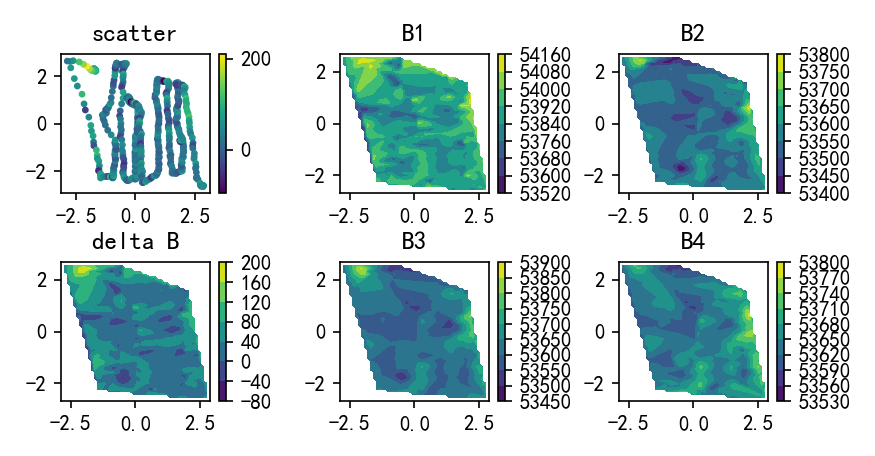
\includegraphics[scale=0.7]{no_item.png}
    \caption{无待测物体时的图例}
    \label{fig:no_item}
\end{figure}

\begin{figure}[h]
    \centering
    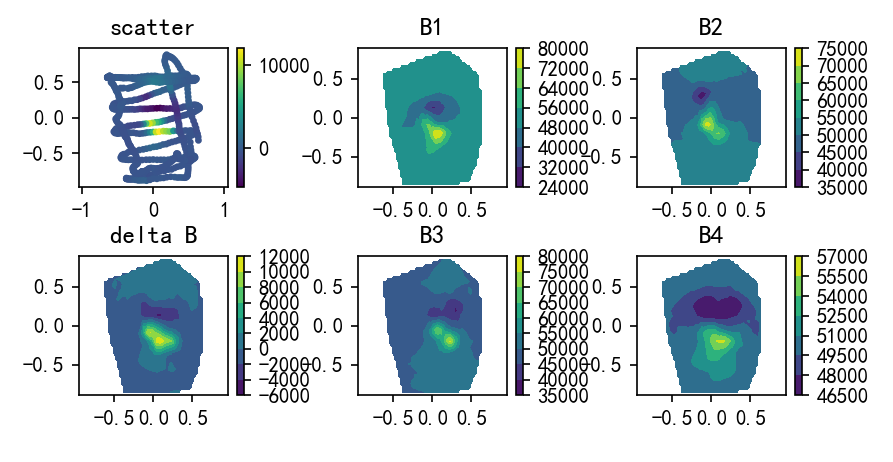
\includegraphics[scale=0.7]{with_item.png}
    \caption{有待测物体时的图例}
    \label{fig:with_item}
\end{figure}

\noindent \textbf{在有目标的数据图像中指出目标的大致位置:}

在图像中标记出磁场强度最大、最小的点,那么他们连线中点即为我们所认为的待测物体位置,
由此我们绘图如图\ref{fig:item}所示,最终我们得到的待测物体坐标为: $[0.08977 -0.02968]$

\begin{figure}[h]
    \centering
    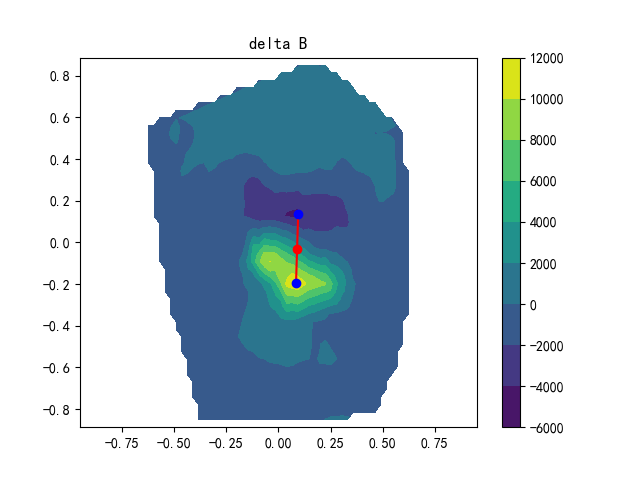
\includegraphics[scale=0.7]{delta B2.png}
    \caption{对待测物体位置的标注}
    \label{fig:item}
\end{figure}



\end{document}